% !TEX program = pdflatex
% Presentation superviseur -- Week 9 -- 2026-06-04
% Version AUTONOME : se lit sans le contexte Week 7/8.
% Structure : Champ -> Questions -> Métrique -> Plafonds -> Méthodes -> Résultats -> Stratégies retenues -> Vers GNN

\documentclass[aspectratio=169,10pt]{beamer}

\usepackage[utf8]{inputenc}
\usepackage[T1]{fontenc}
\usepackage[french]{babel}
\usepackage{lmodern}
\usepackage{booktabs}
\usepackage{array}
\usepackage{tikz}
\usepackage[table]{xcolor}
\usepackage{graphicx}
\usetikzlibrary{positioning, arrows.meta, shapes.geometric, fit, backgrounds, calc}

\usetheme{Madrid}
\usecolortheme{seahorse}
\setbeamertemplate{navigation symbols}{}
\setbeamertemplate{footline}[frame number]
\setbeamerfont{footnote}{size=\tiny}

\definecolor{accent}{RGB}{41, 92, 155}
\definecolor{accentsoft}{RGB}{230, 238, 247}
\definecolor{warn}{RGB}{200, 80, 40}
\definecolor{ok}{RGB}{30, 130, 70}
\definecolor{artcol}{RGB}{41, 92, 155}
\definecolor{jpcol}{RGB}{47, 111, 79}
\definecolor{crosscol}{RGB}{110, 60, 130}

\newcommand{\keybox}[1]{%
  \begin{center}
  \colorbox{accentsoft}{\parbox{0.92\linewidth}{\centering #1}}
  \end{center}}
\newcommand{\warnbox}[1]{%
  \begin{center}
  \colorbox{red!10}{\parbox{0.92\linewidth}{\centering #1}}
  \end{center}}
\newcommand{\okbox}[1]{%
  \begin{center}
  \colorbox{green!10}{\parbox{0.92\linewidth}{\centering #1}}
  \end{center}}
\newcommand{\crossbox}[1]{%
  \begin{center}
  \colorbox{violet!10}{\parbox{0.92\linewidth}{\centering #1}}
  \end{center}}

\title[KG juridique FR --- Week 9]{Construction d'un Knowledge Graph juridique français}
\subtitle{Point d'avancement --- Week 9 : base claire des résultats avant la phase GNN}
\author{Matthieu Kaeppelin}
\institute{Stage FE Recherche}
\date{4 juin 2026}

\begin{document}

% ============================================================
\begin{frame}
  \titlepage
\end{frame}

\begin{frame}{Plan de la séance}
  \tableofcontents[hideallsubsections]
\end{frame}

% ============================================================

% ============================================================
\section{Évaluation : trois métriques complémentaires}

\begin{frame}{Trois métriques, trois angles}
  \footnotesize
  Toutes les métriques sont calculées \textbf{séparément} pour les articles et les JP,
  avec $K = 10$. Notation : \textbf{GT} = \emph{ground truth} (= ce qu'on attend comme réponse),
  $R_{1..K}$ = top-$K$ retourné par la méthode après re-rank cosinus.

  \vspace{0.5em}
  \begin{center}
  \renewcommand{\arraystretch}{1.3}
  \setlength{\tabcolsep}{6pt}
  \begin{tabular}{@{}l p{6cm} p{4cm}@{}}
    \toprule
    \textbf{Métrique} & \textbf{Ce qu'elle évalue} & \textbf{Signal} \\
    \midrule
    \textbf{M1} -- Recall@K & \textit{Combien} de la GT a-t-on retrouvée dans le top-$K$ ? & couverture brute \\
    \textbf{M2} -- Rang moyen normalisé & \textit{À quel rang} la GT apparaît-elle dans le top-$K$ ? & qualité du re-rank \\
    \textbf{M3} -- LLM-as-judge & \textit{Combien des $K$ articles retournés sont pertinents, proches, non pertinents} ? & qualité intrinsèque \\
    \bottomrule
  \end{tabular}
  \end{center}

  \vspace{0.7em}
  \keybox{M1 et M2 mesurent la \textbf{conformité à la GT} (annotation source). M3 ne dépend pas
  de la GT : un LLM juge directement la pertinence sémantique de chaque article retourné.
  Les trois sont nécessaires : M1 seul peut être trompé par un re-rank médiocre, M2 par une GT
  petite, M3 capte ce que la GT ignore.}
\end{frame}

\begin{frame}{Notation des trois métriques}
  \scriptsize

  \begin{block}{\small M1 -- Recall@K \hfill \textit{couverture brute}}
  \vspace{-0.3em}
  \[
    M_1 = \frac{|R_{1..K} \cap \mathrm{GT}|}{|\mathrm{GT}|}
    \qquad
    \text{Plafond} = \frac{\min(|\mathrm{GT}|, K)}{|\mathrm{GT}|}
  \]
  \end{block}

  \begin{block}{\small M2 -- Rang moyen normalisé \hfill \textit{qualité du re-rank}}
  \vspace{-0.3em}
  Pour $a \in \mathrm{GT}$, $\mathrm{rank}(a) \leq K$ si trouvé, sinon $K{+}1$.
  \[
    x = \tfrac{1}{|\mathrm{GT}|}\!\!\sum_{a \in \mathrm{GT}}\!\! \mathrm{rank}(a)
    \qquad
    f(x) = \frac{x - (K{+}1)}{\tfrac{b'+1}{2} - (K{+}1)}, \ b' = \min(|\mathrm{GT}|, K)
  \]
  $f(K{+}1) = 0$ (pire), $f(\tfrac{b'+1}{2}) = 1$ (meilleur).
  \end{block}

  \begin{block}{\small M3 -- LLM-as-judge (Gemma 4 26B) \hfill \textit{qualité intrinsèque}}
  \vspace{-0.3em}
  Score $s_i \in \{0,1,2\}$ par article retourné. Agrégation = \textbf{triplet}.
  \[
    M_3 = (n_2, n_1, n_0), \qquad n_2 + n_1 + n_0 = K
  \]
  Pas de moyenne : $(5,0,5)$ et $(0,10,0)$ moyenne $= 1$ mais qualitativement opposés.
  \end{block}
\end{frame}

\begin{frame}{Distribution de la GT sur la cohorte 977}
  \scriptsize
  \centering
  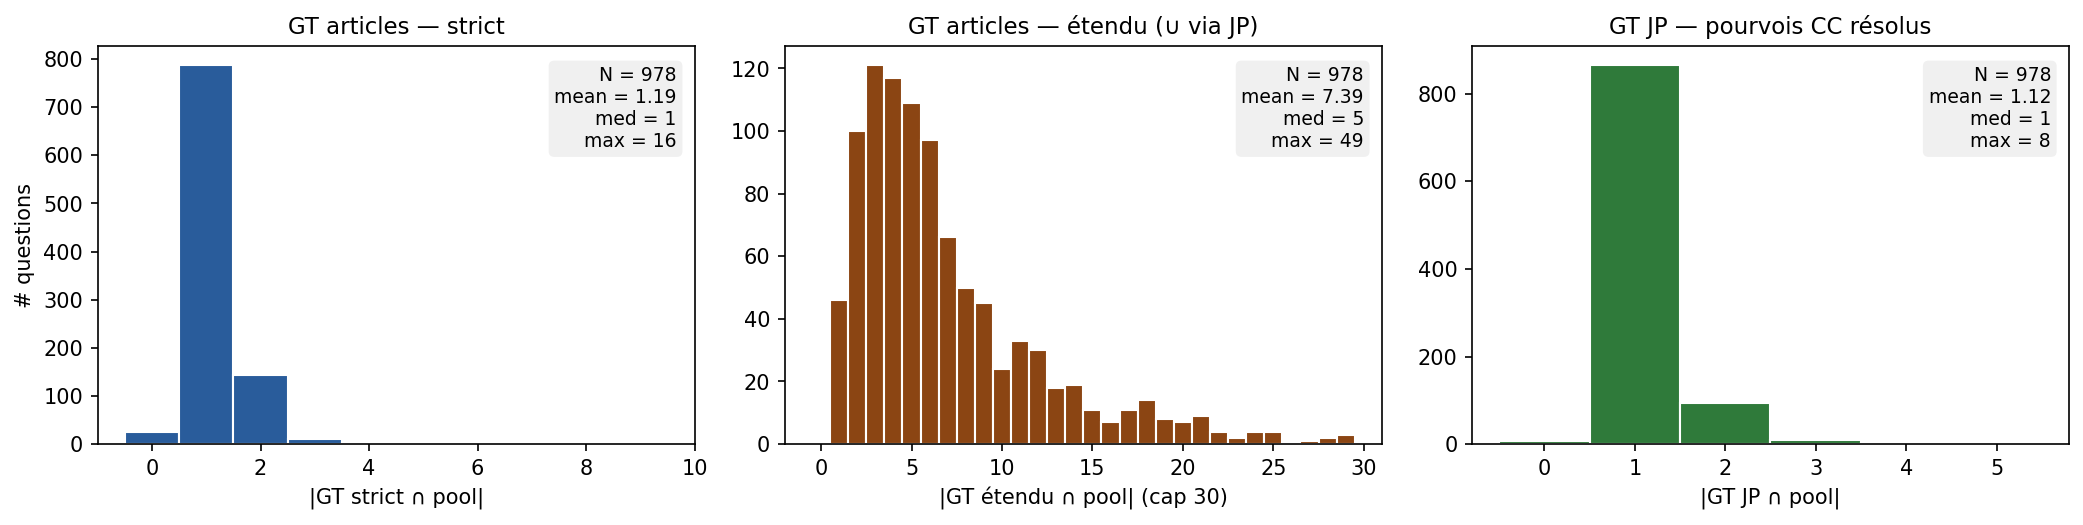
\includegraphics[width=\linewidth]{../../05-Technique/benchmark/etape1_embedding_pur/data/global_bench/fig_hist_977_gt}

  \vspace{0.2em}
  \begin{columns}[T]
    \column{0.33\textwidth}
    \scriptsize\textbf{Articles strict} -- moy. $1{,}19$, médiane $1$, max $16$.
    Court : la fiche source cite peu d'articles.

    \column{0.33\textwidth}
    \scriptsize\textbf{Articles étendu} ($\cup$ via JP $\cap$ graphe v5) -- moy. $7{,}39$, médiane $5$, max $49$.
    Long : la jurisprudence cite beaucoup.

    \column{0.33\textwidth}
    \scriptsize\textbf{JP CC résolu} -- moy. $1{,}12$, médiane $1$, max $8$.
    Pourvois bien formés trouvés dans Judilibre.
  \end{columns}

  \vspace{0.3em}
  \keybox{\scriptsize\textbf{Strict} = ce que la fiche source cite. \textbf{Étendu} = pertinence
  par transitivité jurisprudentielle. La vérité humaine est entre les deux.}
\end{frame}

\begin{frame}{Plafonds M1 -- oracle après filtrage GT $\cap$ pool}
  \scriptsize
  \textbf{Plafond M1} = score que ferait un \emph{retriever idéal} qui ne ramène que les éléments de la GT,
  après qu'on a retiré ceux absents du pool indexé.

  \vspace{0.5em}
  \begin{center}
  \renewcommand{\arraystretch}{1.2}
  \setlength{\tabcolsep}{8pt}
  \begin{tabular}{@{}l c r r@{}}
    \toprule
    \textbf{Modalité} & $K$ & $|\mathrm{GT}|$ moy. & \textbf{Plafond M1} \\
    \midrule
    Articles strict  & 10 & 1,23 & \textbf{100,0 \%} \\
    Articles étendu  & 10 & 7,39 & \textbf{92,8 \%} \\
    JP CC résolu     & 10 & 1,13 & \textbf{100,0 \%} \\
    \bottomrule
  \end{tabular}
  \end{center}

  \vspace{0.5em}
  \begin{flushleft}
  \tiny\textit{Note méthodologique.} Le plafond étendu à $92{,}8~\%$ vient des cas où $|\mathrm{GT}| > K$
  (jusqu'à $49$ articles tous indexés) : par définition $\mathrm{Recall@}K = |R \cap \mathrm{GT}| / |\mathrm{GT}|$
  ne peut alors pas atteindre $1$. Variante \emph{Hit@K} ($|R \cap \mathrm{GT}| / \min(|\mathrm{GT}|, K)$) donnerait
  $100~\%$ partout mais perdrait l'info \og il restait des articles GT hors du top-10 \fg{}. On garde le
  \textbf{Recall@K} classique et on assume le plafond $<100~\%$ sur l'étendu.
  \end{flushleft}
\end{frame}

% ============================================================
\section{Les 4 baselines testées}

\begin{frame}{Quatre familles de méthodes -- 11 variantes}
  \scriptsize
  \renewcommand{\arraystretch}{1.05}
  \setlength{\tabcolsep}{4pt}
  \begin{tabular}{@{}c l p{8.5cm}@{}}
    \toprule
    \textbf{Code} & \textbf{Nom} & \textbf{Idée} \\
    \midrule
    \multicolumn{3}{@{}l@{}}{\textit{\textbf{Baseline 1} -- approche naïve, démontrée cassée et abandonnée}} \\
    B1   & embedding JP entière + mean pooling & \textcolor{warn}{multilingual-e5-base, chunking+pool dilue le signal $\to$ rang médian gold $= 76\,782 / 118\,112$} \\
    \midrule
    \multicolumn{3}{@{}l@{}}{\textit{\textbf{Baseline 2} -- embedding des articles}} \\
    B2-a & cosine pool ouvert      & top-$K$ articles sur les 31~357 articles tous codes \\
    B2-b & cosine pool pénal strict & top-$K$ articles sur les 3~603 articles des 4 codes pénal principaux \\
    \midrule
    \multicolumn{3}{@{}l@{}}{\textit{\textbf{Baseline 3} -- embedding des synthèses LLM des JP}} \\
    B3-a & cosine direct synthèses JP & top-$K$ JP par cosine sur \texttt{emb\_jp\_synthese} (116~755 JP) \\
    B3-b & Art $\to$ JP via graphe & top-$K_{\text{in}}$ articles (B2) $\to$ JP citantes $\to$ re-rank cosinus $\to$ top-$K$ \\
    B3-e & JP $\to$ Art via graphe & top-$K_{\text{in}}$ JP (B3-a) $\to$ articles cités $\to$ re-rank cosinus $\to$ top-$K$ \\
    \midrule
    \multicolumn{3}{@{}l@{}}{\textit{\textbf{Baseline 4} -- cross-modal (combinaison des 2 espaces d'embedding)}} \\
    B4-a & cross-union articles    & articles top-$K_{\text{in}}$ B2 $\cup$ articles top-$K_{\text{in}}$ B3-e \\
    B4-b & cross-inter articles    & articles top-$K_{\text{in}}$ B2 $\cap$ articles top-$K_{\text{in}}$ B3-e \\
    B4-c & cross-union JP          & JP top-$K_{\text{in}}$ B3-a $\cup$ JP top-$K_{\text{in}}$ B3-b \\
    B4-d & cross-inter JP          & JP top-$K_{\text{in}}$ B3-a $\cap$ JP top-$K_{\text{in}}$ B3-b \\
    B4-e & RRF JP (B3-a $+$ B3-b)  & $\mathrm{score}(j) = \sum_i \frac{1}{60 + \mathrm{rank}_i(j)}$ -- fusion par rang, paramètre standard \\
    B4-f & JP pondérée \# citations & union $\cup$ triée par \# top-$K_{\text{in}}$ articles citants \\
    \bottomrule
  \end{tabular}

  \vspace{0.3em}
  \keybox{Toutes les méthodes sauf B1 utilisent \textbf{BGE-M3} (encodeur partagé). B1 est conservé
  comme point de repère historique (palier 7, échec démasqué) mais ne sera pas re-rapporté.}
\end{frame}

% ============================================================
\section{Résultats}

\begin{frame}{Résultats côté ARTICLES -- 971 questions, $K{=}10$}
  \scriptsize
  \textit{Cohorte 977 (option A) : $\ge 1$ article ET $\ge 1$ pourvoi CC résolu dans Judilibre,
  cohorte évaluée = 971 questions (7 CRFPA à ré-encoder). GT strict = \texttt{articles\_attendus} ;
  GT étendu = strict $\cup$ articles cités par les JP attendues via graphe v5.}

  \vspace{0.4em}
  \renewcommand{\arraystretch}{1.1}
  \setlength{\tabcolsep}{4pt}
  \begin{center}
  \begin{tabular}{@{}l l c | r r | r r@{}}
    \toprule
    & & & \multicolumn{2}{c|}{\textbf{GT strict}} & \multicolumn{2}{c}{\textbf{GT étendu}} \\
    \textbf{Var.} & \textbf{Méthode}
    & $K_{\text{in}}$
    & \textbf{M1} & \textbf{M2}
    & \textbf{M1} & \textbf{M2} \\
    \midrule
    B2-a & cosine art. pool ouvert        & --     & 0,459 & 0,369 & 0,185 & 0,172 \\
    \midrule
    \rowcolor{accentsoft}
    B3-e & JP $\to$ Art via graphe        & 10     & \textbf{0,711} & \textbf{0,593} & \textbf{0,399} & \textbf{0,355} \\
    \rowcolor{accentsoft}
    B3-e & JP $\to$ Art via graphe        & 20     & 0,688 & 0,556 & 0,357 & 0,315 \\
    \rowcolor{accentsoft}
    B3-e & JP $\to$ Art via graphe        & 50     & 0,655 & 0,516 & 0,312 & 0,276 \\
    \midrule
    B4-a & cross-union art. (= B2-a)      & 10/20/50 & 0,459 & 0,369 & 0,185 & 0,172 \\
    \bottomrule
  \end{tabular}
  \end{center}

  \vspace{0.5em}
  \okbox{\scriptsize\textbf{Les JP sont un bon point d'entrée pour trouver les articles.}
  B3-e ($K_{\text{in}}{=}10$) domine sur les 4 métriques : M1 strict $71{,}1~\%$, M2 strict $59{,}3~\%$.
  \emph{Intuition} : une JP pertinente est sur le \textbf{même sujet} que la question, et chaque JP
  cite un \textbf{petit nombre} d'articles -- donc passer par les JP filtre le bruit. B4-a $\equiv$ B2-a :
  l'union re-rankée par cosinus dégénère sur le top cosinus initial.}
\end{frame}

\begin{frame}{Résultats côté JP -- 971 questions, $K{=}10$}
  \scriptsize
  \textit{GT JP = pourvois CC résolus dans Judilibre (GT strict $=$ GT étendu côté JP).}

  \vspace{0.3em}
  \renewcommand{\arraystretch}{1.0}
  \setlength{\tabcolsep}{4pt}
  \begin{center}
  \begin{tabular}{@{}l l c | r r@{}}
    \toprule
    \textbf{Var.} & \textbf{Méthode} & $K_{\text{in}}$ & \textbf{M1} & \textbf{M2} \\
    \midrule
    B3-a & cosine direct synthèses JP    & --   & 0,408 & \textbf{0,338} \\
    \midrule
    B4-c & cross-union JP                & 20   & 0,408 & 0,339 \\
    B4-d & cross-inter JP                & 50   & 0,348 & 0,293 \\
    B4-f & union pondérée \# citations   & 10   & 0,154 & 0,103 \\
    \midrule
    \rowcolor{accentsoft}
    B4-e & RRF (B3-a + B3-b)             & 20   & \textbf{0,416} & 0,303 \\
    \bottomrule
  \end{tabular}
  \quad\tiny\textit{($K_{\text{in}}$ $\in \{10, 20, 50\}$ testés, meilleur affiché)}
  \end{center}

  \vspace{0.2em}
  \warnbox{\scriptsize\textbf{Art $\to$ JP via graphe seul est mauvais.}
  Article structurant cité par milliers de JP $\Rightarrow$ voisinage \textbf{bruité}.
  B4-c $\equiv$ B3-a, B4-d $<$ B3-a, B4-f s'effondre (remonte les \emph{grands arrêts populaires}).}

  \vspace{0.2em}
  \okbox{\scriptsize\textbf{B4-e RRF : $0{,}416$ vs B3-a $0{,}408$.}
  Premier gain du graphe côté JP : fusion par \emph{rang} (pas par score), combine confirmation
  cosine + confirmation graphe sans que les outliers dominent. M2 plus bas $\Rightarrow$ plus de GT
  captée mais moins bien classée.}
\end{frame}

% ============================================================
\section{Stratégies retenues et qualité}

\begin{frame}{Stratégies retenues et qualité atteinte}
  \scriptsize
  \textit{Cohorte 977 (option A) -- 971 questions évaluées, $K = 10$.
  Toutes les valeurs sont mesurées après filtrage GT $\cap$ pool.}

  \vspace{0.4em}
  \renewcommand{\arraystretch}{1.2}
  \setlength{\tabcolsep}{4pt}
  \begin{center}
  \begin{tabular}{@{}p{2.4cm} l | r r | r r@{}}
    \toprule
    & & \multicolumn{2}{c|}{\textbf{GT strict}} & \multicolumn{2}{c}{\textbf{GT étendu}} \\
    \textbf{Usage} & \textbf{Méthode retenue}
    & \textbf{M1} & \textbf{M2} & \textbf{M1} & \textbf{M2} \\
    \midrule
    \multicolumn{6}{@{}l@{}}{\textit{Côté articles}} \\
    \rowcolor{accentsoft}
    Champion            & B3-e Art via JP ($K_{\text{in}}{=}10$)  & \textbf{0,711} & \textbf{0,593} & \textbf{0,399} & \textbf{0,355} \\
    Baseline cosine     & B2-a art. pool ouvert                   & 0,459 & 0,369 & 0,185 & 0,172 \\
    \midrule
    \multicolumn{6}{@{}l@{}}{\textit{Côté JP}} \\
    \rowcolor{accentsoft}
    Nouveau champion    & B4-e RRF ($K_{\text{in}}{=}20$)         & \textbf{0,416} & 0,303 & --- & --- \\
    Baseline forte      & B3-a cosine direct synthèses JP         & 0,408 & \textbf{0,338} & --- & --- \\
    \bottomrule
  \end{tabular}
  \end{center}

  \vspace{0.5em}
  \okbox{\scriptsize\textbf{Lecture sur plafond M1 $= 100~\%$ (strict articles et JP).}
  B3-e tient \textbf{7/10 de la GT strict articles} au top-10. B3-a tient \textbf{4/10 de la GT JP}.
  Les deux champions partagent la même brique : \textbf{embeddings BGE-M3 des synthèses JP}.}

  \vspace{0.3em}
  \warnbox{\scriptsize\textbf{Marges restantes.} Articles étendu $39{,}9~\%$ sur plafond $92{,}8~\%$
  (couverture transitive partielle). JP $41{,}6~\%$ sur plafond $100~\%$. \textbf{Phase GNN} :
  exploiter explicitement la structure du graphe pour combler la marge -- premier signal
  positif avec B4-e RRF ($+0{,}8$~pt vs B3-a) mais marge $\sim 60~\%$ à reprendre.}
\end{frame}

% ============================================================
\section{Vers la phase 2 -- GNN comme système de recommandation}

\begin{frame}{Phase 2 -- GNN comme système de recommandation}
  \footnotesize
  \textbf{Idée} : on a 977 questions étiquetées (GT articles + JP CC). On les ajoute au graphe comme
  troisième type de nœud, et on entraîne un modèle à \textbf{prédire les arêtes} question $\to$ article
  et question $\to$ JP.

  \vspace{0.3em}
  \begin{center}
  \scalebox{0.72}{
  \begin{tikzpicture}[node distance=0.4cm,
      art/.style={circle,fill=artcol!20,draw=artcol,thick,minimum size=0.55cm,inner sep=0pt,font=\tiny},
      jp/.style={rectangle,fill=jpcol!20,draw=jpcol,thick,minimum size=0.55cm,inner sep=0pt,font=\tiny},
      q/.style={diamond,fill=crosscol!20,draw=crosscol,thick,minimum size=0.65cm,inner sep=0pt,font=\tiny}]
    \node[art] (a1) at (0, 1.5)    {A$_1$};
    \node[art] (a2) at (0, 0.75)   {A$_2$};
    \node[art] (a3) at (0, 0)      {A$_3$};
    \node[art] (a4) at (0, -0.75)  {A$_4$};
    \node[jp]  (j1) at (4, 1.5)    {JP$_1$};
    \node[jp]  (j2) at (4, 0.75)   {JP$_2$};
    \node[jp]  (j3) at (4, 0)      {JP$_3$};
    \node[jp]  (j4) at (4, -0.75)  {JP$_4$};
    \node[q]   (q1) at (2, 1.9)    {Q$_1$};
    \node[q]   (q2) at (2, -1.15)  {Q$_2$};
    \draw[gray, thin] (a1) -- (j1);
    \draw[gray, thin] (a1) -- (j2);
    \draw[gray, thin] (a2) -- (j2);
    \draw[gray, thin] (a3) -- (j3);
    \draw[gray, thin] (a4) -- (j4);
    \draw[crosscol, thick, dashed] (q1) -- (a1);
    \draw[crosscol, thick, dashed] (q1) -- (j1);
    \draw[crosscol, thick, dashed] (q1) -- (j2);
    \draw[crosscol, thick, dashed] (q2) -- (a4);
    \draw[crosscol, thick, dashed] (q2) -- (j4);
    \node at (0, -1.4)  {\tiny Articles};
    \node at (4, -1.4)  {\tiny Jurisprudences};
    \node at (2, 2.4)   {\tiny Questions (nouveau type de n\oe uds)};
  \end{tikzpicture}}
  \end{center}

  \vspace{0.2em}
  \keybox{\textbf{Analogie système de recommandation} -- (utilisateur, film) $\to$ (question, \{article, JP\}).
  Trois types de n\oe uds + relations typées (citation Art$\leftrightarrow$JP, GT-article, GT-JP).
  Cadre technique : \textbf{link prediction sur graphe hétérogène}. \textbf{Démarrage simple} :
  Personalized PageRank depuis la question (zéro entraînement, inductif natif), puis montée
  progressive vers LightGCN / R-GCN inductif si signal positif.}
\end{frame}

\begin{frame}{Phase 2 -- plan de travail proposé}
  \footnotesize
  \textbf{Pré-requis empiriques à mesurer} :
  connectivité (composante géante, distance Q $\to$ GT) ; distribution des degrés (hubs déjà
  toxiques sur B4-c/B4-f) ; couverture GT dans pool ($\sim$97~\% art., $\sim$99~\% JP CC, déjà OK).

  \vspace{0.3em}
  \textbf{Plan court terme} :
  \begin{itemize}\setlength\itemsep{0.05em}
    \item \textbf{S10} : Personalized PageRank depuis Q (seeds = top-$K$ BGE-M3). Zéro entraînement, inductif natif.
    \item \textbf{S11} : LightGCN sur Q$\to$\{Art, JP\} (BPR loss), splits par question.
    \item \textbf{S12} : R-GCN inductif si LightGCN positif.
  \end{itemize}

  \vspace{0.3em}
  \textbf{Référence à battre} ($K{=}10$, 971 questions) :
  B3-e art. strict $0{,}711/0{,}593$ ; art. étendu $0{,}399/0{,}355$ ; B4-e JP $0{,}416/0{,}303$.

  \vspace{0.3em}
  \crossbox{\scriptsize\textbf{Concurrent à benchmarker} : cross-encoder \texttt{BAAI/bge-reranker-v2-m3}
  sur top-30 de B3-e / RRF $\to$ ré-ordonnance top-10. Simple, rapide, souvent compétitif --
  fixe une vraie référence avant tout GNN.}
\end{frame}

\begin{frame}{PPR -- problèmes anticipés \& diagnostic préalable}
  \scriptsize
  \begin{tabular}{@{}p{2.7cm} p{4.4cm} p{4.4cm}@{}}
    \toprule
    \textbf{Problème} & \textbf{Origine} & \textbf{Parade} \\
    \midrule
    Hubs Art$\to$JP & Art structurants (1240, 1382\ldots) cités par $5{\,}000{+}$ JP
                    & Normalisation symétrique $P[i,j] = 1/\sqrt{d_i d_j}$ ; éventuel cap de degré \\
    Convergence lente & Diamètre du graphe $\sim 6$, multi-hop
                      & 20--30 itérations, monitorer $\|r^{t+1}-r^t\|$ \\
    Choix de $\alpha$ & Trop bas $\Rightarrow$ PPR $\approx$ cosine seul ;
                       trop haut $\Rightarrow$ propagation dans les hubs
                      & Sweep $\alpha \in \{0{,}3 ; 0{,}5 ; 0{,}7 ; 0{,}85 ; 0{,}95\}$,
                        séparément Art / JP \\
    Choix du seed     & Q seule ? Q $+$ top-$K$ cosine ? top-$K$ uniquement ?
                      & 3 variantes à tester ; pondération par similarité cosine \\
    Articles hors pool & Graphe $= 87{\,}821$ articles, pool BGE-M3 $= 31{\,}357$
                       & Filtrer le ranking PPR au pool indexé (déjà fait pour M1/M2) \\
    \bottomrule
  \end{tabular}

  \vspace{0.5em}
  \textbf{Diagnostic graphe à exécuter avant PPR} (script \texttt{20\_graph\_stats.py}) :
  \begin{itemize}\setlength\itemsep{0.05em}
    \item Composante géante (\% nœuds) -- $<95~\%$ $\Rightarrow$ alerte
    \item Distribution des degrés Art (P50, P95, P99) -- $P_{99}^{art} > 10\,000$ $\Rightarrow$ hubs problématiques
    \item Distribution des degrés JP (P50, P95, P99) -- $P_{99}^{jp} > 50$ $\Rightarrow$ JP catch-all
    \item Distance médiane Q $\to$ GT (via seeds cosine $+$ citations) -- $> 3$ hops $\Rightarrow$ PPR convergera mal
  \end{itemize}

  \vspace{0.3em}
  \keybox{\scriptsize\textbf{Lecture de l'optimum $\alpha^*$} : si $\alpha^*$ proche de 0 $\Rightarrow$
  le graphe n'apporte rien au-delà du cosine. Si $\alpha^*$ proche de 1 $\Rightarrow$ le graphe contient
  l'essentiel du signal. Diagnostic en soi, avant tout LightGCN.}
\end{frame}

\begin{frame}{PPR naïf -- premiers résultats (cohorte 971, $K{=}10$)}
  \scriptsize
  Seed $=$ top-10 cosine articles $\cup$ top-10 cosine JP, poids $=$ similarité.
  Power iteration 20 steps, sweep $\alpha$, deux normalisations testées.

  \vspace{0.3em}
  \renewcommand{\arraystretch}{1.1}
  \setlength{\tabcolsep}{4pt}
  \begin{center}
  \begin{tabular}{@{}l c | r r r r | r r@{}}
    \toprule
    \textbf{Norm.} & $\alpha$
    & \multicolumn{2}{c}{\textbf{Art. strict}} & \multicolumn{2}{c|}{\textbf{Art. étendu}}
    & \multicolumn{2}{c}{\textbf{JP}} \\
     & & M1 & M2 & M1 & M2 & M1 & M2 \\
    \midrule
    row & 0,50 & 0,514 & 0,471 & 0,246 & 0,269 & 0,409 & \textbf{0,342} \\
    row & 0,70 & 0,563 & 0,484 & 0,348 & 0,363 & 0,408 & 0,337 \\
    \rowcolor{accentsoft}
    row & 0,85 & 0,601 & 0,445 & \textbf{0,421} & \textbf{0,412} & 0,411 & 0,320 \\
    \midrule
    sym & 0,85 & 0,462 & 0,423 & 0,187 & 0,206 & 0,409 & 0,335 \\
    \midrule
    \multicolumn{2}{l|}{B3-e Art via JP}
                  & \textbf{0,711} & \textbf{0,593} & 0,399 & 0,355 & --- & --- \\
    \multicolumn{2}{l|}{B4-e RRF JP}
                  & --- & --- & --- & --- & \textbf{0,416} & 0,303 \\
    \bottomrule
  \end{tabular}
  \end{center}

  \vspace{0.2em}
  \okbox{\scriptsize\textbf{Signal positif côté étendu.} PPR row $\alpha{=}0{,}85$ bat B3-e
  sur articles étendu ($+2{,}2$ pts M1, $+5{,}7$ pts M2) \textbf{sans entraînement}, et égale
  B4-e côté JP. Le graphe contient bien du signal exploitable au-delà du re-rank cosinus.}

  \vspace{0.2em}
  \warnbox{\scriptsize\textbf{Sym-normalize collapse au cosine seul.} La matrice symétrique
  n'est pas stochastique $\Rightarrow$ la masse décroît à chaque step, seul le seed survit.
  Adapté à LightGCN (sommation multi-couches), pas à PPR. \textbf{On garde row-normalize.}}

  \vspace{0.2em}
  \crossbox{\scriptsize\textbf{À explorer ensuite (résultats à venir)} :
  \textit{(a)} sweep $K_{\text{in}} \in \{5, 10, 20, 50\}$ ;
  \textit{(b)} variantes seed (Art seul, JP seul, Art$+$JP) ;
  \textit{(c)} cap de degré ou anti-hub heuristique côté articles structurants (1240, 1382\ldots).}
\end{frame}

\begin{frame}{PPR -- courbes diagnostic (convergence \& sweep $\alpha$)}
  \scriptsize
  \centering
  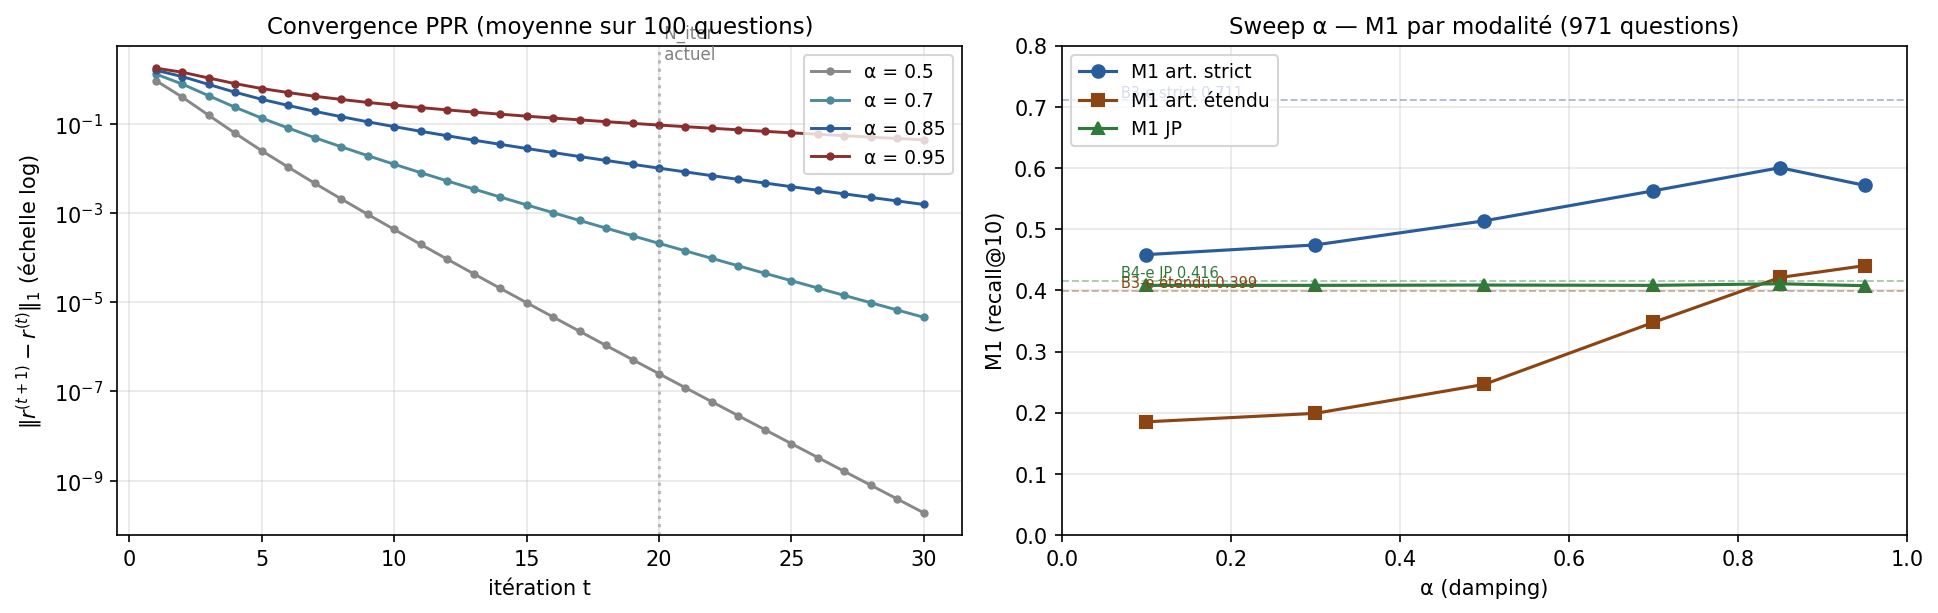
\includegraphics[width=0.99\linewidth]{../../05-Technique/benchmark/etape1_embedding_pur/data/global_bench/fig_ppr_curves}

  \vspace{0.2em}
  \begin{columns}[T]
    \column{0.48\textwidth}
    \scriptsize\textbf{Gauche : convergence}.
    Résidu $\|r^{(t+1)} - r^{(t)}\|_1$ par itération, moyenne 100 questions. À $\alpha{=}0{,}5$
    on converge en $\sim 10$ steps ; à $\alpha{=}0{,}85$, encore $\sim 10^{-4}$ à $t{=}20$ ;
    à $\alpha{=}0{,}95$, $\sim 10^{-3}$. Le \textbf{$N_{\text{iter}}$ actuel (20)} est OK pour
    $\alpha \leq 0{,}85$, à pousser à 30+ pour $\alpha{=}0{,}95$.

    \column{0.48\textwidth}
    \scriptsize\textbf{Droite : sweep $\alpha$}.
    Articles strict : maximum à $\alpha{=}0{,}85$ (0,601). Articles étendu : monte jusqu'à
    $\alpha{=}0{,}95$ (\textbf{0,441 vs 0,421}). JP : insensible à $\alpha$ (toujours $\sim 0{,}41$).
    $\Rightarrow$ \textbf{optimum dépend de la modalité} ; aller plus loin que $0{,}85$ aide pour
    la transitivité graphe (étendu) mais dégrade la précision strict.
  \end{columns}
\end{frame}

\begin{frame}{PPR -- où va la masse}
  \scriptsize
  \centering
  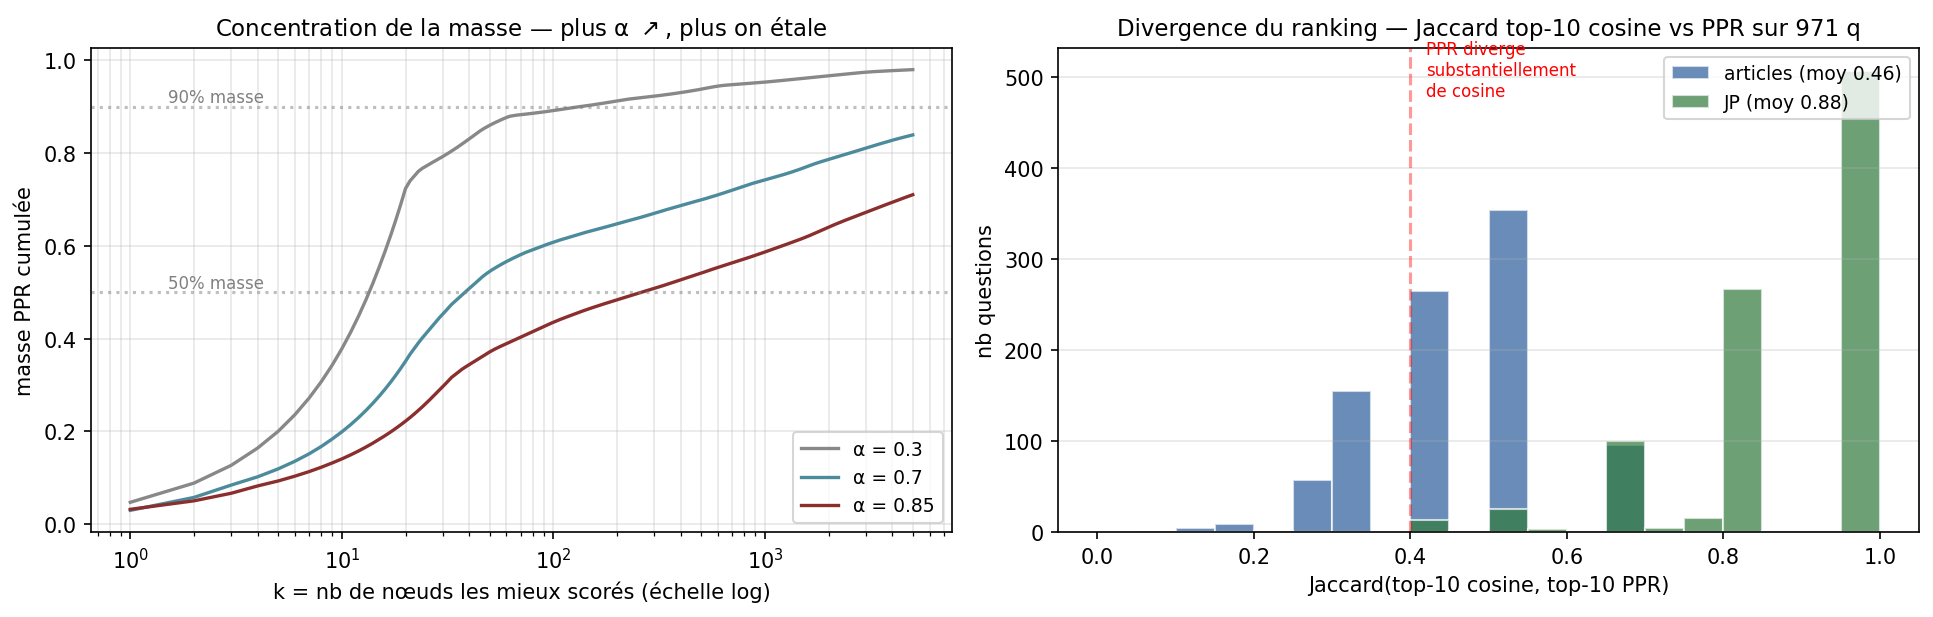
\includegraphics[width=0.99\linewidth]{../../05-Technique/benchmark/etape1_embedding_pur/data/global_bench/fig_ppr_weights}

  \vspace{0.4em}
  \begin{columns}[T]
    \column{0.48\textwidth}
    \scriptsize\textbf{Gauche -- Concentration de la masse.}
    À $\alpha{=}0{,}3$, $50~\%$ de la masse PPR est sur $\sim 10$ nœuds (proche du seed cosine).
    À $\alpha{=}0{,}85$, il faut $\sim 100$ nœuds pour atteindre $50~\%$ : PPR \emph{étale} la masse
    sur le voisinage graphe, c'est exactement la diffusion attendue.

    \column{0.48\textwidth}
    \scriptsize\textbf{Droite -- Divergence ranking.}
    Jaccard$(\text{top-}10_{\text{cosine}}, \text{top-}10_{\text{PPR}})$ sur 971 questions.
    \textbf{Articles : méd. 0,43} $\Rightarrow$ PPR change $\sim 6$ articles sur 10.
    \textbf{JP : méd. 1,00} $\Rightarrow$ PPR ne change presque rien côté JP, ce qui explique
    le gain nul vs B4-e.
  \end{columns}
\end{frame}

% ============================================================
\section{Discussion}

\begin{frame}{Questions ouvertes pour la discussion}
  \footnotesize
  \begin{enumerate}\setlength\itemsep{0.5em}
    \item \textbf{Validation humaine} -- les 6 questions pénal de CRFPA ont un gold structuré
    (core/expected/expert), absent dans \texttt{doctrine\_qgen}. On valide notre métrique sur ce
    sous-corpus humain en S10 ?

    \item \textbf{Élargir la résolution gold JP} -- aujourd'hui $43{,}1$ \% des questions sont hors champ
    JP (pourvoi non résolvable). Matcher CA/TJ par n° de rôle + ECLI passerait à $\sim 80$ \% de couverture.
    Priorité avant ou après le GNN ?

    \item \textbf{Métrique unique vs deux colonnes (strict / étendu)} -- on garde la double lecture
    (transparence) ou on fixe une définition pour S10+ ?

    \item \textbf{Cross-encoder avant GNN} -- baseline forte à benchmarker en S10 : si elle atteint
    déjà recall $\geq 0{,}6$ / précision $\geq 15$ \% à $K{=}10$, le GNN devient marginal.

    \item \textbf{Extension benchmark hors pénal} -- étendre \texttt{doctrine\_qgen} à civil / admin /
    social en parallèle du chantier GNN, ou consolider d'abord le pénal ?
  \end{enumerate}
\end{frame}

\begin{frame}
  \begin{center}
    \vspace{2em}
    {\Large\textbf{Merci.}}
    \vspace{2em}

    \textit{Discussion / questions}

    \vspace{2em}
    \scriptsize
    Branche : \texttt{etape1-embedding-pur}\\
    Journal : \texttt{01-Projet/journal/2026-05-28.md}\\
    Scripts : \texttt{05-Technique/benchmark/etape1\_embedding\_pur/scripts/}\\
    \texttt{13\_eval\_recall\_at\_k.py}, \texttt{14\_histogram\_gold\_size.py}, \texttt{16\_score\_plafonds.py}
  \end{center}
\end{frame}

\end{document}
